\chapter{转换对象与校验方法}\label{ch:objects}
\section{样例说明}
样例以文献\cite{shannon1948}演示引用格式，不把文献内容作为测试数值的来源。参数 $a=2$ 与 $b=3$ 用于数学对象的编辑性检查。图\ref{fig:demo}和表\ref{tab:demo}分别展示排版用的图像与数据。\footnote{这是脚注转换测试，内容不属于实际研究。}
\section{公式与符号}
线性关系示例见式\eqref{eq:linear}。
\begin{equation}\label{eq:linear}
\mathbf{y}=\begin{bmatrix}1&2\\3&4\end{bmatrix}\mathbf{x}+\mathbf{n}
\end{equation}
式中，$\mathbf{x}$ 为示例输入向量；$\mathbf{n}$ 为示例附加项。归一化指标的数学排版见式\eqref{eq:ratio}。
\begin{equation}\label{eq:ratio}
e=\frac{\sum_{i=1}^{N}(x_i-\hat{x}_i)^2}{\sum_{i=1}^{N}x_i^2}
\end{equation}
\section{图表}
\begin{figure}[htbp]\centering
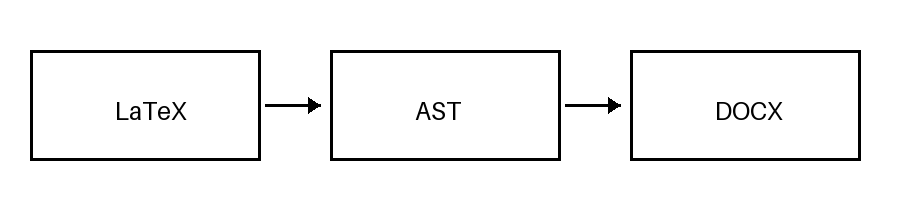
\includegraphics[width=0.65\linewidth]{diagram.png}
\caption{文档转换验证流程}\label{fig:demo}
\end{figure}
\begin{table}[htbp]\centering
\caption{排版测试数据}\label{tab:demo}
\begin{tabular}{ccc}\toprule
对象 & 输入值 & 输出值\\\midrule
甲 & 2 & 4\\
乙 & 3 & 9\\\bottomrule
\end{tabular}
\end{table}
表中的数值是明确标注的演示值，不能用于论文结果。
\section{本章小结}
本章给出转换所需的基本对象及标签，下一章检查跨章引用和条件表达。
